%%% A chip (or possibly multichip) architecture that support the easy movement of data from
%%% memory or IOs to the accelerators based on an ``identified data flow model''. Emphasis
%%% should be on redefining cache based architectures so that they address both sparse and
%%% dense data sets. Integration of the processor and memory architecture may be necessary.


%%% An external memory controller which is designed to ensure efficient us of the identified
%%% ``data mapping tools''. The controller should be able to efficiently handle random as well as
%%% sequential memory accesses. Every effort should be made to minimize the size of the data
%%% access to avoid the need to pad memory. The use of advanced memory technology may
%%% be necessary

%%% How will you design a memory controller to take advantage of the data maps?
%%% The key to efficient processing of large scale graph analytics is to ensure the locality of
%%% information. The less you have to move the data, the more efficient the computation from both a
%%% power and performance perspective. The memory controller needs to exploit locality regardless
%%% of whether the dataset is sparse or dense.

\noindent
Our preliminary study exhibits that the memory bandwidth utilization is very low for many graph algorithms.
This is because these algorithms often require random/sparse memory accesses, whereas the memory hierarchy is optimized only for sequential/dense memory accesses.
The study also shows that we must re-design the entire memory hierarchy if we are going to effectively support both random/sparse and sequential/dense memory accesses.
That is, optimizing either on-chip caches or off-chip memory alone is ineffective.
Thus, we propose to architect the GAMA memory system, consisting of (1) a private L1 cache for each corelet, (2) a shared spatially-temporally boosted eDRAM cache across all corelets within a GAMA tile, and (3) 32GB of DiRAM4, to efficiently support random/sparse and sequential/dense memory accesses.
More specifically, it will be built on circuit/architecture techniques and a soon-to-be-released DRAM technology and achieve the target 90\% utilization of memory bandwidth. 

\noindent
\subsubsection{Off-Chip Memory Architecture.} 
\label{sec:memory:off-chip}
\noindent
\textbf{Memory technology.} 
We will use  Tezzaron's DiRAM4 for the main memory of each GAMA tile.  
Each DiRAM4 die provides 8GB capacity with 64$\times$32-bit ports (total 2048 I/O pins) with 1TB/s bandwidth. 
HBM2 is expected to provide the same bandwidth as DiRAM4, but we choose DiRAM4 because it provides narrower but more memory channels than HBM2 (16$\times$128-bit channels). 
We believe that DiRAM is more advantageous than HBM2 for graph algorithms that generate random/sparse memory accesses. 
Each tile integrates 4$\times$8GB DiRAM modules and thus there is a total of 4TBps internal memory bandwidth between the GAMA core and the main memory within each tile. 


\vspace{3pt}
\noindent
\textbf{Memory controller.} 
We propose a memory controller architecture supporting dynamic memory channel reconfigurations to effectively support both random/sparse and sequential/dense accesses.
By default the GAMA main memory system starts with many narrow memory channels to efficiently service random/sparse memory accesses.
However, it can be dynamically chained a subset of 64 physical memory channels to form wider logical memory channels to efficiently service sequential/dense memory accesses, depending on current memory access patterns. 
For sequential/dense accesses, multiple small memory requests can be merged (coalesced) into one single memory request, allowing more efficient utilization of the memory scheduling queue.
Meanwhile, when narrow memory channels are fused into a wide (logical) memory channel, we have more memory scheduling queue entries in a memory controller.
These two aspects improve the utilization of both command/address and data buses for sequential/dense memory accesses.


To dynamically configure the memory channels, we exploit the information from the provided datamap that is stored for each matrix and large front-end memory queues. 
The datamap enables the memory controller to infer how consecutive elements of a row or column (irrespective of whether the matrix is dense or sparse) are laid out. 
The front-end memory queue buffers requests from corelets across the entire GAMA system, as all GAMA tiles see a globally shared address space (see \textbf{``Memory model''}). 
The memory queue monitors requests from multiple corelets and identifies all the requests that are bound to a given bank or channel. 
It will then pull all the data from a single channel that may satisfy multiple corelet requests.  

To enable efficient coalescing the memory queue may delay memory requests for a short interval that does not affect the utilization of processing pipeline and memory channel. 
As each GAMA tile computes over a small slice of compressed vectors (or a slice of a row or column in a dense matrix) we expect that memory requests from different corelets within each tile may exhibit spatial locality. 
Even sparse matrix representations will exhibit strong spatial locality across row or column values that are used in a given matrix operation.  Thus the front-end memory queue buffers requests and extracts spatial locality by coalescing memory requests to  
Note that the traditional memory queues cannot be large because they rely on CAM.
Instead of CAM-based memory queue, we aim to architect the large memory queue using a structure like set-associative cache, where entries are indexed by memory request address ranges to confirm the full matching after comparing the tags associated with the index.
A list structure associated with the memory queue keeps track of valid entries in the cache-like structure based on a scheduling policy and sends the entries to the back-end memory queues associated with each DRAM bank.

\vspace{3pt}
\noindent
\textbf{Memory model.} 
The GAMA system will adopt a distributed shared memory model with non-uniform memory access latency. 
Hence, all the 16 GAMA tiles will share the address space. The programer uses OpenCAPI protocol to launch a sparse matrix operation on the GAMA accelerator. OpenCAPI provides  the libcxl library for initiating accelerator launch and memory management APIs, such as $cxl\_afu\_open\_dev$ to open the accelerator and $cxl\_afu\_attach$ to start the accelerator. The data for the accelerator is placed in a work element descriptor (WED) and is passed as a pointer to GAMA. The accelerator and P8 share the same virtual memory space. By default the data is interleaved across the tiles at the granularity of 128MB. This interleaving allows significant amount of contiguous matrix data to be placed per each tile, while at the same time allowing a large matrix to be mapped across multiple tiles to improve memory parallelism.   
 
% and there will be no virtual memory support.  
%M - do we need to say we don't support virtual memory? I think NUMA and virtual memory are orthogonal issues.
%The host OpenPower system uses memory-mapped I/O to access the GAMA system. 
%Hence, the entire DiRAM4 will be mapped to higher order virtual address space of the host OpenPower system. 
%M - earlier you stated that there will be no virtual memory support.
%The programer uses a simple host-accelerator protocol to launch a sparse matrix operation on the GAMA system. 

%%%%NAM - need to revise and how to leverage CAPI.


\vspace{3pt}
\noindent
\textbf{Data placement.} 
By default the data is interleaved across all tiles at the granularity of 128MB. 
%M - why 128MB?
Each 128MB data slice may be further interleaved in various banks and channels within each tile.  
Given the criticality of memory latency and bandwidth to graph processing, we will provide several higher-level software APIs to allow the application developer or compilers (T2 thrust) to provide semantic information about matrix representations laid out in memory. 
For instance, the programmer may explicitly tag the column pointer, row index and value vectors (for compressed column representation). 
This information will be used by the memory system to determine how to layout these arrays (bank interleaving and distribution across memory channels) in memory and also to generate bank and channel access commands for each vector appropriately. 
% intermediate matrices and vectors that may be generated  may also be tagged by the programmer to indicate how they are being stored (doubly compressed column or row etc.,).  %For instance, in centrality analysis using all pairs shortest paths approach the shortest paths for each pair are stored as intermediate results that will be used in the final reduction process to extract the central vertex.  Each matrix or vector's  physical address to appropriate bank and channel activation sequence.
%Appropriate interleaving of data across a large number of channels is critical for enabling parallel access. 
%If requests from multiple GAMA corelets can be routed to different channels then their requests can be satisfied in parallel. 
Depending on the sparse matrix representation some data structures may see sequential accesses to large blocks while other structures may encounter mostly random accesses. For instance, in a compressed column  representation the column pointer vector is randomly accessed to select a given column (for instance, in a BFS the starting vertex column) and then the value in column pointer is used as index into row index  vector and value vector. The row index and value vectors are scanned together to reconstruct the column. Hence it is best to put the row index vector and value vector on different channels which can be concurrently accessed to accelerate the column reconstruction.  

For dense matrices we expect the programmer to use the software API to provide hints to the hardware whether a matrix is predominantly accessed column-wise or row-wise in the next computation phase. 
These hints can be updated at various computation phases in a kernel. The hardware uses this information to decide on an appropriate matrix layout in memory. 

%MURALI:SHOULD WE INCLUDE THIS LEVEL OF DETAILS?
\vspace{3pt}
\noindent
\textbf{Memory datamap.} 
Once the data (either sparse or dense matrix) is laid out in each GAMA tile's memory, a metadata table (or datamap) will be generated to indicate the row and columns ranges stored at each tile for a given matrix.   
The datamap also stores the  approximate number of non-zero elements in each row and column of a matrix in a distributed manner across multiple tiles. As described later, the sparsity information is used to improve load balancing.     
The metadata may also store finer-granularity information such as the channel and bank interleaving information for rows and columns. 
This metadata information will be used to enable simple optimizations such as gating bank activations when a given DiRAM4 bank is not needed in a computation.    
% During the initial data layout phase each sparse matrix that is laid out in memory will store metadata in the banks to indicate the min and max index values of the various row and column indices that are stored in a given memory bank. This information can be used to determine which banks to activate. For instance if a column X-Y is all zeros in a given row then there is no need to accesss the column vector values of rows X-Y. If X-Y fit in a bank we can disable the bank. 
During a matrix-vector or matrix-matrix (AXB) multiplication, the corelets first construct the row that is currently used in A and then use only the non-zero row indices to fetch the corresponding column elements from B. 
For instance, if column X of a give row is zero then there is no need to fetch the row X value from the column. 
To enable such optimizations the corelet must first construct the non-zero column indices and then use that index vector to disable or enable memory accesses. 

%MURALI: DO WE PROVIDE A PROGRAMMING INTERFACE? OR HOW IS THE MEMORY LAID OUT OTHERWISE? 



%Graph algorithms are typically very memory-intensive while the memory access patterns are very random (i.e., poor sptial and temporal locality).  These characteristics greatly reduce the efficiency of traditional memory systems that are typically optimized for serving sequential memory requests.  For example, running BFS on a GPU, we observe that the memory system becomes the performance bottleneck even when HBM provides 512GB/s.  In this project, we aim to implement a memory system that can support both random and sequential memory accesses for sparse and dense datasets.
 
%The L2 cache line size is 64 bytes. As we will discuss later the cache supports variable granularity  cache line size, which we call elastic cache. Hence, a single 64 line may contain up to four 16-byte chunks from different addresses.  


\subsubsection{On-Chip Cache Architecture.} 
\label{sec:memory:on-chip}
\noindent
\textbf{L1 cache.}
We propose elastic cache architecture to efficiently support both narrow- and wide-width memory accesses from multiple non-contiguous memory locations to co-reside in a single 64-byte cache line. 
Specifically, we introduce a concept of chunk tags to store tags for narrow-width data blocks (e.g., 4-, 8-, or 16-byte byte blocks) along with a conventional tag (referred to as common tag) for each cache line (see Figure~\ref{fig:elastic-cache}). 
Chunk tags add only a small storage overhead. Elastic cache allows us to efficiently use 64-byte cache lines for storing narrow-width data blocks from non-contiguous addresses, that may be seen in sparse matrices, as well as a 64-byte contiguous  blocks that may be seen in dense matrices without significant cache reorganization. 
Note that just adopting narrow cache lines is not efficient to handle sequential memory requests for dense datasets according to our experiments.
Our preliminary study shows this architecture applied to L1 caches of a traditional GPU architecture improve the performance by more than 2$\times$ for SPMV.
We expect that the performance can much further improved when the architecture is also applied to large L2 cache.


%Note that just adopting narrow cache lines is not efficient to handle sequential memory requests for dense datasets according to our experiments.
%Figure~\ref{fig:elastic-cache-flow} describes the access flow of the proposed \texttt{Elastic-Cache}. 
%Note that we will employ the proposed \texttt{Elastic-Cache} architecture for both private SRAM-based L1 and shared eDRAM-based L2 caches.

\begin{wrapfigure}{r}[0pt]{0.4\textwidth}
\center
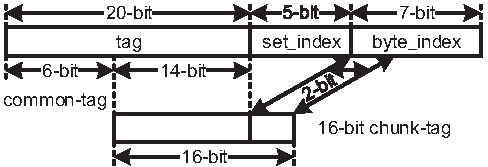
\includegraphics[width=1.0\linewidth]{./fig/chunk_tag_16bit-eps-converted-to.pdf}
\caption{The chunk and common tags to support both narrow- and wide-width on-chip cache accesses for a 4-way 16KB cache.}
\label{fig:elastic-cache}
\end{wrapfigure}

\begin{comment}
\begin{wrapfigure}{r}[0pt]{0.4\textwidth}
\center
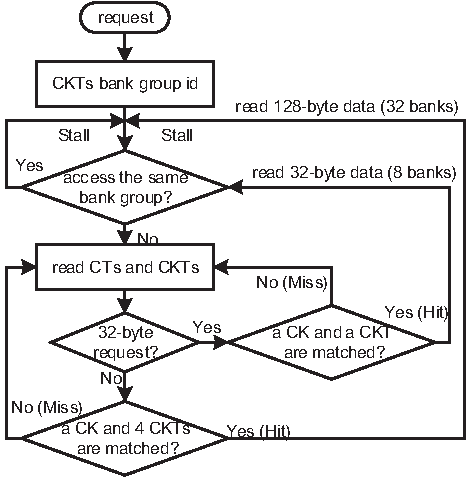
\includegraphics[width=1.0\linewidth]{./fig/flow_chart-eps-converted-to.pdf}
\caption{Access flow of \texttt{Elastic-Cache}. \texttt{CT}, \texttt{CKT}, and \texttt{CK} denote common tag, chunk tag, and chunk.}
\label{fig:elastic-cache-flow}
\end{wrapfigure}
\end{comment}

Considering our corelet architecture with a 16-lane SIMD engine (cf. Section~\ref{sec:processing}), we will architect to architect the elastic L1 cache with 16 banks, each of which is 4KB and provides 4 bytes per cycle. 
This architecture is preferrable, as the 16-lane SIMD engine can simultaneously request 16 memory accesses to different addresses.
The connection between an elastic L1 cache and a corelet is described in Section~\ref{sec:processing}.

\vspace{3pt}
\noindent
\textbf{L2 cache.}
% 10/12 MS edited three paragraphs below. 
%We will implement the L1 and L2 caches using SRAM and eDRAM bitcells. 
The L2 cache is shared amongst 32 GAMA corelets and is implemented using eDRAM. In implementing eDRAM-based L2 cache, we aim to %minimize latency %and support \texttt{Elastic-Cache} data access. 
%In the eDRAM based L2, it is particularly critical to 
overcome relatively long latency of accessing eDRAM cache compared with SRAM cache. 
%In this project, %building upon our recent work on low-energy and compact memory-based FFT core\footnote{ISSCC'17 submitted}, 
We will apply a dynamic fine-grained spatial-temporal voltage boosting technique only on the peripheral circuits (address decoders, multiplexers/demultiplexers, and interconnect buffers), but not bitcells. 
This boosting technique is synergistic with the elastic cache architecture and beneficial for graph algorithms that often need to access a small subset of a large cache line without dissipating excessive power. 
We will explore voltage boosting up to the thermal/reliability-limited level in a temporarily and spatially fine-grained fashion for improving access latency and throughput. 
We will also effectively gate or use low supply voltage (e.g., 0.6V or lower) for the circuits that are not involved in accessing the demand data, making them serve as thermal buffers. 
%This way, we expect to significantly improve latency still under the thermal limit. 
Assuming 0.5V threshold voltage ($V_T$)\footnote{High $V_T$ is common in embedded memory for suppressing leakage}, boosting from 0.8V to 1.4V can increase the overdrive level ($V_{DD}$-$V_T$) from 0.3V to 0.9V, improving latency and throughput by at least 3X. 
The low $V_{DD}$ used in the rest of cache circuits can save a significant amount of leakage energy dissipation. 
By exploiting this latency improvement, we will explore to make the cache systems to perform multiple fine-grained data accesses (in serial by default but in parallel if data are in the multiple banks) and pack and send them back to the pipeline of a corelet. 

\begin{wrapfigure}{r}[0pt]{0.35\textwidth}
\center
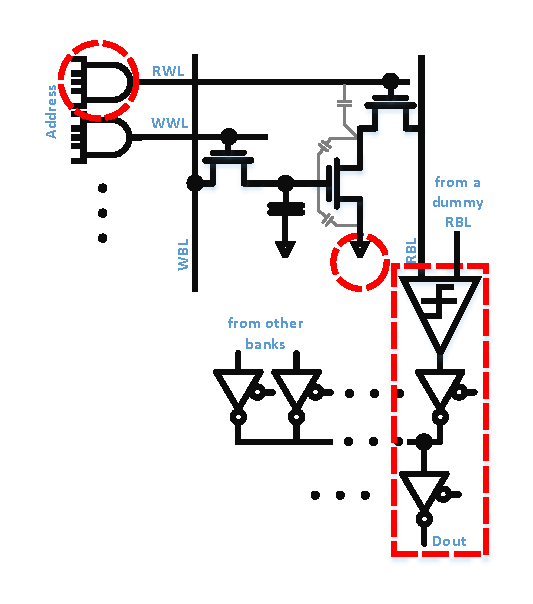
\includegraphics[width=2.4in, trim=20 20 10 50]{./fig/boosting.pdf}
\caption{A boosting scheme for the L2 cache using 3T eDRAM bitcells. Red dashed outlines highlight the portions receiving boosting/underdriving. It is critical to protect dynamic nodes from coupling noises of boosting via parasitic capacitors (gray).}
\label{fig:boosting}
\end{wrapfigure}

To enable such voltage boosting, we need to meet two requirements.  First, we need to boost voltage in a fraction of cycle time. 
This can be achieved first by having strong power-grid for boosted voltage, together with a good amount of decoupling capacitors circuits. 
Still, the power grid, due to the sub-nanosecond transient change, can undergo a non-negligible amount of voltage integrity degradation (i.e., droops, overshoot, and ripples). 
%Over-designing power grids and decoupling capacitors can incur significant area and energy overhead. 
Our approach to this challenge is to apply techniques that tolerate such problems in power grids through in-situ error detection and correction (EDAC), as EDAC can detect and correct timing errors from supply voltage droop without over-design and the worst-case margin. Specifically, we will develop an EDAC technique that primarily focuses on detecting errors and allowing instruction replays to deal with error correction.

Second, we need small and precise thermal monitoring systems to stop voltage overdrive if temperature rises above a temperature limit. 
Note that existing state-of-the-art in on-chip thermal monitoring, however, have been limited due to sensor circuits that are too invasive in terms of size ($>$ a few thousand $\mu m^2$ per sensor) and voltage-scalability (requiring $>$ 1V). 
This limitation prevents sensors from being placed closely to digital hotspots. 
In this project, we will create improved thermal monitoring systems for embedded memory based on our recent thermal sensor designs that achieves about two orders of magnitude more compact (30 $\mu m^2$ per sensor), comparably or more accurate ($\pm 1.1^oC 3-\sigma$ error), and voltage scalable down to 0.4V \cite{ISSCC14, JSSC15, CICC15}. 
%By placing such sensors closely to estimated hotspots, we anticipate to achieve high accuracy in thermal monitoring, which will allow us to use voltage boosting longer and more frequently without pessimistic throttling. 
Furthermore in eDRAM caches, accurate thermal sensing will be used to adaptively change the refresh cycles, saving energy and increasing access availability. 

\begin{comment}
To enable such voltage boosting, we need to meet two requirements. 
First, we need to boost voltage in a fraction of cycle time. 
This can be achieved first by having strong power-grid for boosted voltage, together with a good amount of decoupling capacitors circuits. 
Still, the power grid, due to the sub-nanosecond transient change, can undergo a non-negligible amount of voltage integrity degradation (i.e., droops, overshoot, and ripples). 
Over-designing power grids and decoupling capacitors can incur significant area and energy overhead. 
Our approach to this challenge is to apply techniques that tolerate such problems in power grids, specifically in-situ error detection and correction (EDAC)
%\footnote{MICRO'02 \& JSSC'06}. 
EDAC can detect and correct timing errors from supply voltage droop without over-design and the worst-case margin. 
Conventional EDAC works, however, have focused on in-order pipelines, not embedded memory, and used instruction replay based correction which may not be suitable for caches having no instruction equivalent. 
Stopping a shared cache for correction can also increase latency, degrading the throughput of the whole accelerator. 
In this project, therefore, we will create EDAC techniques applicable to embedded memory. 
%In recent works, we created new EDAC techniques for specialized and parallelized architectures in near/sub-$V_T$ circuits, 
%including correction schemes based on body swapping and voltage boosting, which do not need instruction replay. 
We will extend our previous works with a key focus of enabling non-instruction replay based correction for near/super-$V_T$ circuits. 
Our initial direction is to leverage our sparse error-detector insertion scheme.%\footnote{ISLPED'14,TVLSI'16 (pending)}. 
In our study, the sparse insertion framework suggests circuit delay increases incurred by dynamic variations would not develop explicit timing errors at super-$V_T$ (>0.55V in 65nm) as long as such increases do not accumulate. 
This implies that if we can clean up delay accumulation sufficiently quickly by changing $V_{DD}$, the load can operate at the edge of the first failure without having explicitly developed errors. 
In addition, we will explore to take advantage of a unique characteristics of embedded memory that are relevant to EDAC, namely the narrow distribution of read/write path delay, i.e., it takes almost the same delay to access any row. 
We plan to take advantage of this and explore an EDAC technique based on pulsed latches. 
The narrow path delay distribution can enable a small to a moderate amount of short path padding while providing a good amount of cycle borrowing. 
We can leverage the low-cost pulsed-latch sequencing
%\cite{jin_asscc16} 
for reducing error-detector overhead.

Second, we need to stop voltage overdrive if temperature rises above a temperature limit. 
To do this, we need precise thermal monitoring systems. 
Existing arts in on-chip thermal monitoring, however, have been limited due to sensor circuits that are too invasive in terms of size ($>$ a few thousand $\mu m^2$ per sensor) and voltage-scalability (requiring $>$ 1V). 
This limitation prevents sensors from being placed closely to digital hotspots\footnote{ISSCC’12}. 
The resulted non-negligible distance between sensors and hotspots increases thermal monitoring error in the range of 10$^oC$ to 20$^oC$. 
%\footnote{TACO’08, DAC'12}. 
In this project, therefore we will create better thermal monitoring systems for embedded memory. 
We will build upon our recent sensor circuits
%\footnote{ISSCC’14, JSSC’15, CICC’15} 
that are very compact (30 $\mu m^2$/sensor) and voltage-scalable to share digital supply voltages. 
By placing such sensors closely to estimated hotspots, we anticipate to achieve high accuracy in thermal monitoring, which will allow us to use voltage boosting longer and more frequently without pessimistic throttling. 
Furthermore in eDRAM caches, this will help a refreshing scheme to adaptively change refreshing periods, saving energy and increasing access availability. 
\end{comment}

\begin{comment}
To overcome relatively long latency of accessing eDRAM compared to SRAM, we propose to apply a dynamic fine-grained spatial voltage boosting technique to eDRAM-based L2 \texttt{Elastic-Cache}. 
This boosting technique is synergistic with \texttt{Elastic-Cache} and beneficial for graph algorithms that only need to access a small subset of a large eDRAM cache line without dissipating excessive power.
Especially, we will explore voltage boosting all the way to the thermal-limited level in a temporarily and spatially fine-grained fashion for improving access latency and throughput. 
We will also effectively gate or lower supply voltage of the circuits that are not involved in accessing the interested data, making them serving as thermal buffers. 
This way, we expect to significantly improve latency still under the thermal limit. 
In addition, exploiting the latency improvement, we will explore to make the cache systems to perform multiple fine-grained data accesses (in serial by default but in parallel if data are in the multiple banks) and pack and send them back to the pipeline of a graph accelerator. 


To enable such voltage boosting, one of the key requirements is to stop voltage overdrive if temperature rises above a temperature limit. 
To do this, we need precise thermal monitoring systems. 
Existing arts in on-chip thermal monitoring, however, have been limited due to sensor circuits that are too invasive in terms of size (> a few thousand µm2 per sensor) and voltage-scalability (requiring > 1V). 
This limitation prevents sensors from being placed closely to digital hotspots (ISSCC’12). 
The resulted non-negligible distance between sensors and hotspots increases thermal monitoring error in the range of 10 to 20oC (TACO’08). 
In this project, therefore we will create better thermal monitoring systems for eDRAM. 
We will build upon our recent sensor circuits (ISSCC’14, JSSC’15, CICC’15) that are very compact (30µm2/sensor) and voltage-scalable to share digital supply voltages. 
By placing such sensors closely to estimated hotspots, we can achieve high accuracy in thermal monitoring, which will allow us to use voltage boosting longer and more frequently without pessimistic throttling. 
Furthermore this will help a refreshing scheme to adaptively change refreshing periods, saving energy and increasing access availability in eDRAM. 


\noindent
\textbf{Off-chip Memory Architecture:} 
We aim to build our memory sub-system on Tezzaron's DiRAM4 3D Memory for the main memory of our accelerator. 
One 8GB DiRAM die provides 64 32-bit ports (total 2048 I/O pins) with 1TB/s bandwidth. 
HBM2 is expected to provide the same bandwidth as DiRAM, but we choose DiRAM because DiRAM provides narrower but more memory channels (64×32-bit channels) than HBM2 (16×128-bit channels). 
That is DiRAM is more advantageous than HBM2 for graph algorithms that generate random/irregular memory accesses. 

Especially, we will introduce a concept of dynamic memory channel configuration to the memory controllers so that we can dynamically use these 64 physical memory channels to form narrower or wider logical memory channels to efficiently service both random/irregular and sequential/regular memory accesses from the accelerators, depending on current memory access patterns. 
To dynamically configure the memory channels we exploit the information from the provided ``data-map'' and large front-end memory queues (or also known as holding buffer).
The front-end memory queue aim to coalesce as many random/irregular memory requests as possible by holding memory requests as long as possible in a degree that does not affect the utilization of processing pipeline and memory channel.
Note that the traditional memory queues cannot be large because they rely on CAM.
Instead of CAM-based memory queue, we aim to architect the large memory queue using a structure like set-associative cache, where entries are indexed by memory request addresses and confirms the full matching after comparing the tags associated with the index.
A list structure associated with the memory queue keeps track of valid entries in the cache-like structure based on a scheduling policy and sends the entries to the back-end memory queues associated with each DRAM bank.
\end{comment}
